\chapter{Conception de l'intelligence artificielle} \label{chapter:intelligence-artificielle}

Pour la conception de l'intelligence artificielle, nous avons fait le choix de la variante nega-max de l'algorithme min-max
avec l'élagae alpha-béta.

Dans ce chapitre, nous rappelons ce qu'est min-max, nega-max et alpha-béta, puis nous présentons nos fonctions d'évaluation
de l'état du plateau (heuristiques).

\section{Rappel de l'algorithme du min-max}

Le min-max est un algorithme visant à minimiser la perte maximum dans le cas d'un jeu à somme nulle
et informations complètes pour deux joueurs. On cherche donc à
maximiser son gain tandis que l'adversaire cherche à le minimiser (autrement dit à maximiser le
sien étant donné que le jeu est à somme nulle).
Le principe de l'algorithme est très simple : on parcourt l'arbre de jeu dans le but de faire remonter
à la racine un score qui est associé à la meilleure transition estimée.
Pour cela, on doit distinguer deux types de nœuds : les nœuds max (nœuds joueur) et les nœuds min (nœuds adverse).
Les nœuds min prennent la valeur la plus faible de leurs enfants tandis que les nœuds max prennent la valeur la
plus élevée de leurs enfants.
Pour les feuilles de l'arbre, on évalue l'état correspondant du jeu.

Voici un arbre d'exemple :

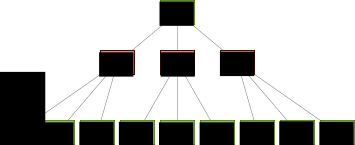
\includegraphics[scale=0.6]{minmax}

Les nœuds verts sont ici des nœuds max et les nœuds rouges des nœuds min.

On voit ici que la transition à choisir est la troisième qui assure d'obtenir un gain de 53 dans le pire des cas.
Même s'il est possible de gagner plus dans d'autres cas, on part du principe que l'adversaire ne nous laissera pas faire.

\section{Nega-max sans élagage}

Il existe une simplification du min-max, le principe restant rigoureusement le même.
L'idée est simplement de toujours prendre l'opposé des valeurs enfants.
En effet : prendre le maximum de l'opposé des valeurs est équivalent à prendre le minimum des valeurs.
Ainsi, il n'est plus nécessaire de gérer trois cas (feuille, min, max), mais seulement deux (feuille, max).

Exemple sur l'arbre précédent :

\includegraphics[scale=0.6]{negamax}

Les résultats sont identiques.

\section{Nega-max avec élagage alpha-béta}

Les algorithmes précédents effectuent une exploration complète de l'arbre alors qu'il est possible de n'effectuer
qu'une exploration partielle de l'arbre en élagant les transitions dont on est sûr que la qualité des solutions générées
sera inférieure ou égale.

Le principe de l'élagage alpha-béta est de garder la trace d'une borne inférieure (\(\alpha\)) et supérieure (\(\beta\))
pour chaque nœud. Lorsque la borne inférieure est supérieure à la borne supérieure, on arrête l'exploration des nœuds frères.
On met à jour la borne inférieure sur les nœuds max et la borne supérieure sur les nœuds min.

Exemple :

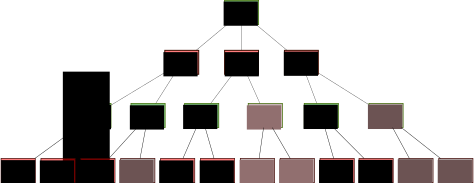
\includegraphics[scale=0.5]{negamax-alphabeta}

Ici, on effectue trois coupures :
\begin{itemize}
    \item le nœud max a été mis à jour à 90 (\(\alpha\) = 90). Comme c'est un nœud max, il ne peut qu'augmenter.
        La valeur de \(\beta\) est à 89. On effectue donc la coupure (\(\alpha > \beta\)).
    \item le nœud min a été mis à jour à 45 (\(\beta\) = 45). Comme c'est un nœud min, il ne peut que diminuer.
        La valeur de \(\alpha\) est à 89. On effectue donc la coupure.
    \item le nœud min a été mis à jour à 15 (\(\beta\) = 15). Comme c'est un nœud min, il ne peut que diminuer.
        La valeur de \(\alpha\) est à 89. On effectue donc la coupure.
\end{itemize}

\section{Heuristiques}

…

\subsection{Facile: win-lose}

…

\subsection{Normal}

…

\subsection{Difficile}

…

\subsection{Légendaire}

…

